% Unofficial University of Cambridge Poster Template
% https://github.com/andiac/gemini-cam
% a fork of https://github.com/anishathalye/gemini
% also refer to https://github.com/k4rtik/uchicago-poster

\documentclass[final]{beamer} 

% ====================
% Packages
% ====================

\usepackage[T1]{fontenc}
\usepackage{lmodern}
\usepackage[orientation=portrait,size=a2,scale=1.05]{beamerposter}
\usetheme{gemini}
\usecolortheme{nott}
\usepackage{graphicx}
\usepackage{booktabs}
\usepackage{tikz}
\usetikzlibrary{arrows.meta,positioning}
\usepackage{pgfplots}
\pgfplotsset{compat=1.14}
\usepackage{anyfontsize}
\usepackage{xurl}


% ====================
% Lengths
% ====================

% If you have N columns, choose \sepwidth and \colwidth such that
% (N+1)*\sepwidth + N*\colwidth = \paperwidth
\newlength{\sepwidth}
\newlength{\colwidth}
\setlength{\sepwidth}{0.025\paperwidth}
\setlength{\colwidth}{0.45\paperwidth}

\newcommand{\separatorcolumn}{\begin{column}{\sepwidth}\end{column}}

% ====================
% Title
% ====================

\title{FlowTM: gemelo digital estocástico para optimizar la operación BRT}

\author{Alvarado B. Ludwig \and Mahecha R. Albert \and Pinilla N. Kevin \and Ospina R. Maria}


% ====================
% Footer (optional)
% ====================

\footercontent{
  Facultad de Ciencias Naturales e Ingeniería \hfill
  XXXII Feria de Proyectos de Aula \hfill
  Inteligencia Artificial}
% (can be left out to remove footer)


% ====================
% Logo (optional)
% ====================

% use this to include logos on the left and/or right side of the header:
\logoright{
\includegraphics[height=2.5cm]{logos/utadeo-logo.png}}




% ====================
% Body
% ====================

\begin{document}

% Refer to https://github.com/k4rtik/uchicago-poster
% logo: https://www.cam.ac.uk/brand-resources/about-the-logo/logo-downloads
% \addtobeamertemplate{headline}{}
% {
% \begin{tikzpicture}[remember picture,overlay]
%   \node [anchor=north west, inner sep=3cm] at ([xshift=-2.5cm,yshift=1.75cm]current page.north west)
%   {\includegraphics[height=7cm]{logos/unott-logo.eps}}; 
% \end{tikzpicture}
% }

\begin{frame}[t]
  \begin{columns}[t]
    \separatorcolumn

    \begin{column}{\colwidth}

      \begin{block}{RESUMEN}

        FlowTM es un gemelo digital físico-estocástico para explorar la operación de un corredor BRT. Integra datos GTFS, validaciones agregadas y un simulador de eventos discretos para evaluar horarios candidatos bajo demanda variable y una flota limitada. Un agente de optimización redistribuye los intervalos de seis servicios y valida la política resultante con semillas fuera de muestra.

      \end{block}

      \begin{block}{OBJETIVOS}

        \begin{itemize}
          \item Construir un escenario reproducible del corredor Portal Norte--Marly a partir de datos GTFS y validaciones.
          \item Evaluar cómo la redistribución de frecuencias afecta la espera, el sobrecupo, los pasajeros varados y la flota.
          \item Comparar el horario GTFS con una alternativa optimizada mediante simulación estocástica y validación holdout.
        \end{itemize}

      \end{block}

      \begin{alertblock}{METODOLOGÍA}

        \textbf{Escenario.} Portal Norte--Marly, sentido sur, 06:00--09:00, 19 estaciones y 18 servicios. Se optimizan H13, H75, H27, J74, K23 y L18 con una cota de flota $B_{\max}=244$ y capacidad asumida de 160 pasajeros por bus.

        \textbf{Simulación.} Las llegadas se generan estocásticamente en ventanas de 15 minutos. El simulador modela colas, destinos, \textit{dwell time}, tiempos de recorrido y reutilización física de buses.

        \textbf{Optimización.} Un agente de búsqueda por recocido simulado propone vectores de \textit{headways} entre 2 y 15 minutos. Se usan 150 evaluaciones, cinco semillas de entrenamiento y 30 semillas \textit{holdout} pareadas con intervalos de confianza del 95\%.

        \begin{figure}[H]
          \centering
          \begin{tikzpicture}[node distance=0.35cm, every node/.style={font=\small, align=center},
            box/.style={draw, rounded corners, fill=blue!8, minimum width=2.3cm, minimum height=0.65cm},
            arrow/.style={-Latex, thick}]
            \node[box] (data) {GTFS +\\validaciones};
            \node[box, right=of data] (scenario) {Escenario\\del corredor};
            \node[box, right=of scenario] (sim) {Simulador\\SimPy};
            \node[box, below=of sim] (eval) {Evaluador\\estocástico};
            \node[box, left=of eval] (agent) {Recocido\\simulado};
            \node[box, left=of agent] (occ) {OCC\\React/MapLibre};
            \draw[arrow] (data) -- (scenario);
            \draw[arrow] (scenario) -- (sim);
            \draw[arrow] (sim) -- (eval);
            \draw[arrow] (eval) -- (agent);
            \draw[arrow] (agent) -- (occ);
            \draw[arrow] (sim.east) |- (occ.south);
          \end{tikzpicture}
          \caption{Flujo de datos, simulación, optimización y visualización.}
          \label{Arquitectura}
        \end{figure}

        \begin{figure}[H]
          \centering
          \begin{tikzpicture}
            \begin{axis}[
              width=0.95\linewidth, height=5.2cm,
              ybar, bar width=8pt, ymin=0, ymax=10,
              ylabel={Buses con sobrecupo (\%)},
              symbolic x coords={Base,Optimizado}, xtick=data,
              nodes near coords, nodes near coords align={vertical},
              enlarge x limits=0.55, grid=major, major grid style={gray!20},
              every axis label/.append style={font=\small},
              tick label style={font=\small}, label style={font=\small}
              ]
              \addplot[fill=blue!55] coordinates {(Base,8.095) (Optimizado,7.5205)};
            \end{axis}
          \end{tikzpicture}
          \caption{Validación holdout: el sobrecupo disminuye de 8.095\% a 7.5205\%.}
          \label{Sobrecupo}
        \end{figure}




      \end{alertblock}

      \begin{block}{RESULTADOS}

        \begin{itemize}
          \item \textbf{Utilidad:} $-2.0243 \rightarrow -2.0063$; $\Delta=+0.0180$, IC 95\% $[+0.0036,+0.0324]$.
          \item \textbf{Sobrecupo:} $8.095\% \rightarrow 7.5205\%$; reducción aproximada del 7.1\%, significativa.
          \item \textbf{Espera media:} $3.5063 \rightarrow 3.5172$ minutos; no se demuestra una reducción.
          \item \textbf{Pasajeros transportados:} $54\,121.8 \rightarrow 54\,112.3$; sin mejora significativa.
          \item \textbf{Flota:} el contraste reporta $244 \rightarrow 243$; la cota operacional sigue siendo $B_{\max}=244$.
        \end{itemize}

        \begin{figure}[H]
          \centering
          \begin{tikzpicture}
            \begin{axis}[
              width=\linewidth, height=6.2cm,
              ybar=0pt, bar width=5pt, ymin=0, ymax=8.5,
              ylabel={Intervalo (min)}, xlabel={Servicio},
              symbolic x coords={H13,H75,K23,J74,H27,L18}, xtick=data,
              xticklabel style={font=\small}, yticklabel style={font=\small},
              legend style={at={(0.5,1.03)}, anchor=south, legend columns=2,
                font=\small}, grid=major, major grid style={gray!20}
              ]
              \addplot[fill=gray!60] coordinates
              {(H13,3.27) (H75,3.75) (K23,4.50) (J74,5.00) (H27,5.45) (L18,6.00)};
              \addplot[fill=orange!75] coordinates
              {(H13,3.27) (H75,4.25) (K23,7.50) (J74,3.50) (H27,3.95) (L18,7.00)};
              \legend{GTFS,Optimizado}
            \end{axis}
          \end{tikzpicture}
          \caption{Redistribución de \textit{headways} en el snapshot validado.}
          \label{Headways}
        \end{figure}

        \vspace{0.3cm}
        \textbf{Lectura principal:} el agente mejora el equilibrio de ocupación y la utilidad, pero el beneficio no es uniforme: la espera media no disminuye y los pasajeros transportados no aumentan significativamente.

      \end{block}  


    \end{column}

    \separatorcolumn   


    \begin{column}{\colwidth}

      \begin{figure}[H]
        \centering
        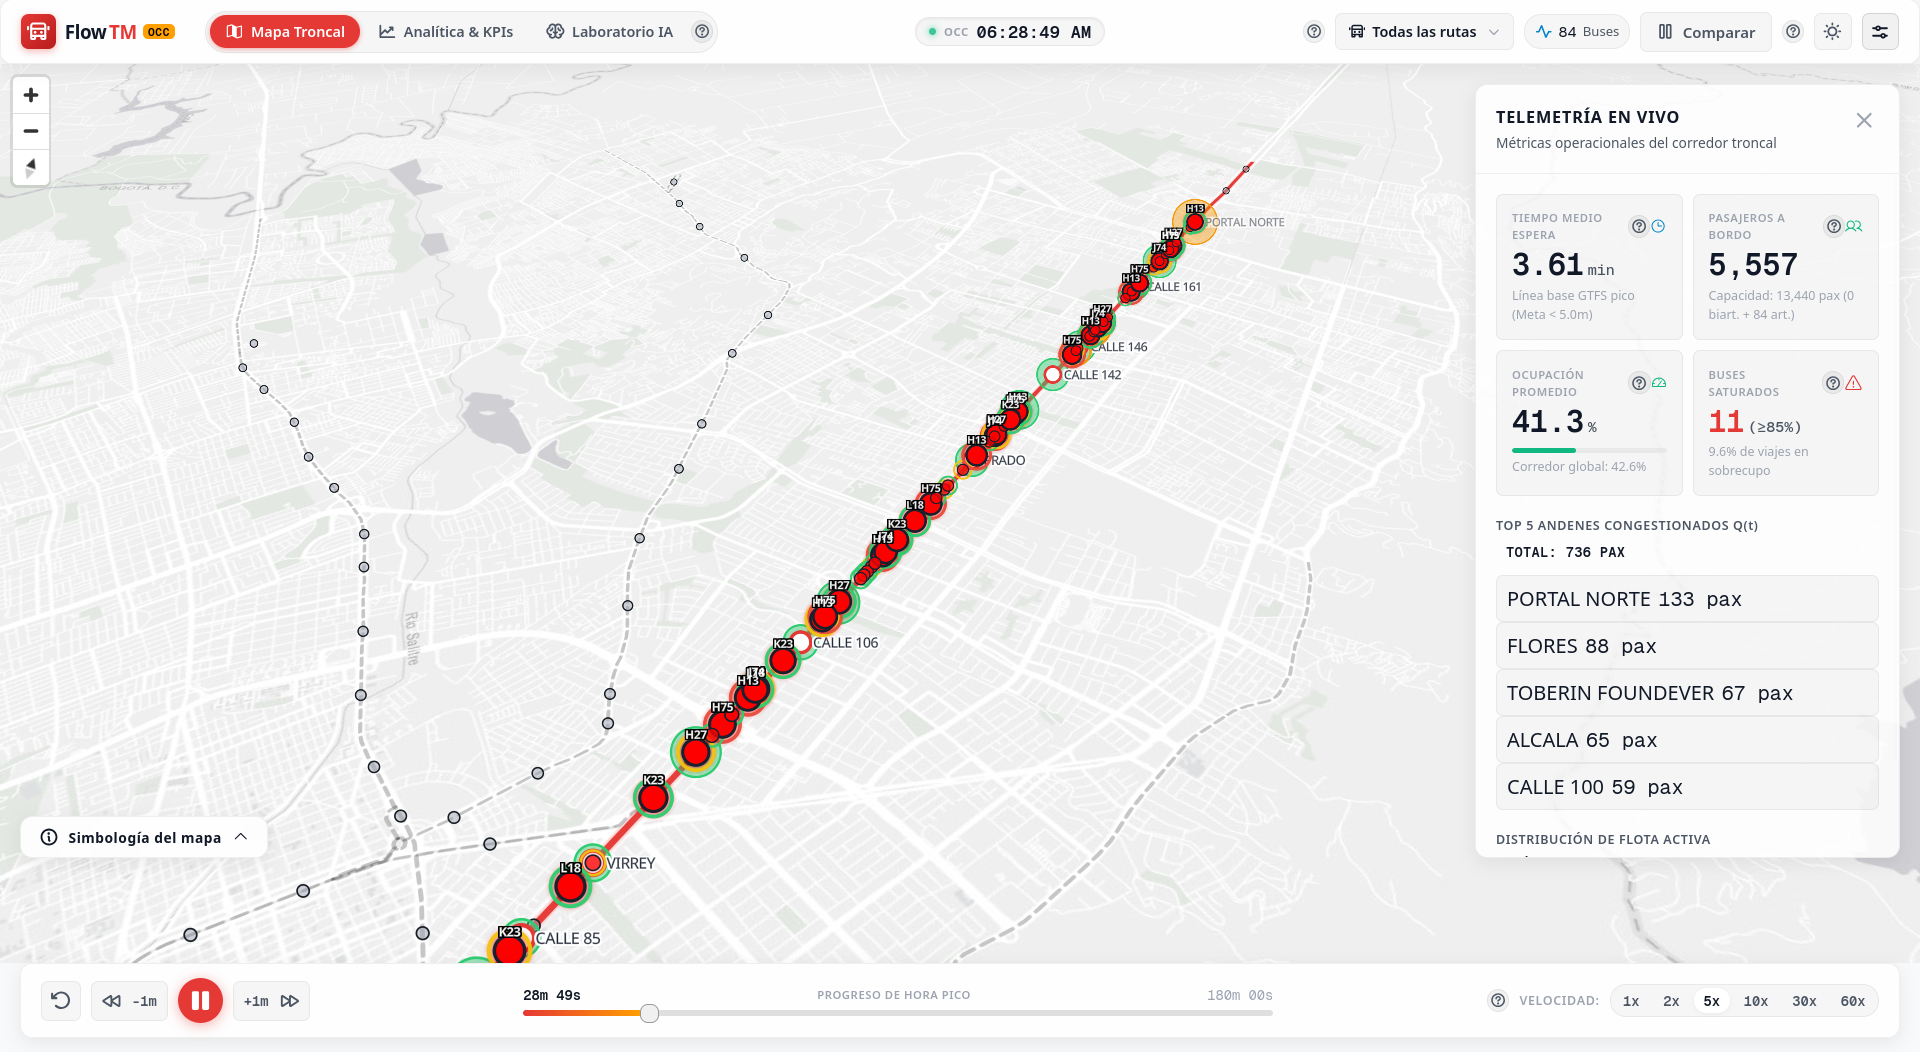
\includegraphics[width=\textwidth]{img/dash.png}
        \caption{Visualizador de rutas}
        \label{visualizador}
      \end{figure}

      \begin{figure}[H]
        \centering
        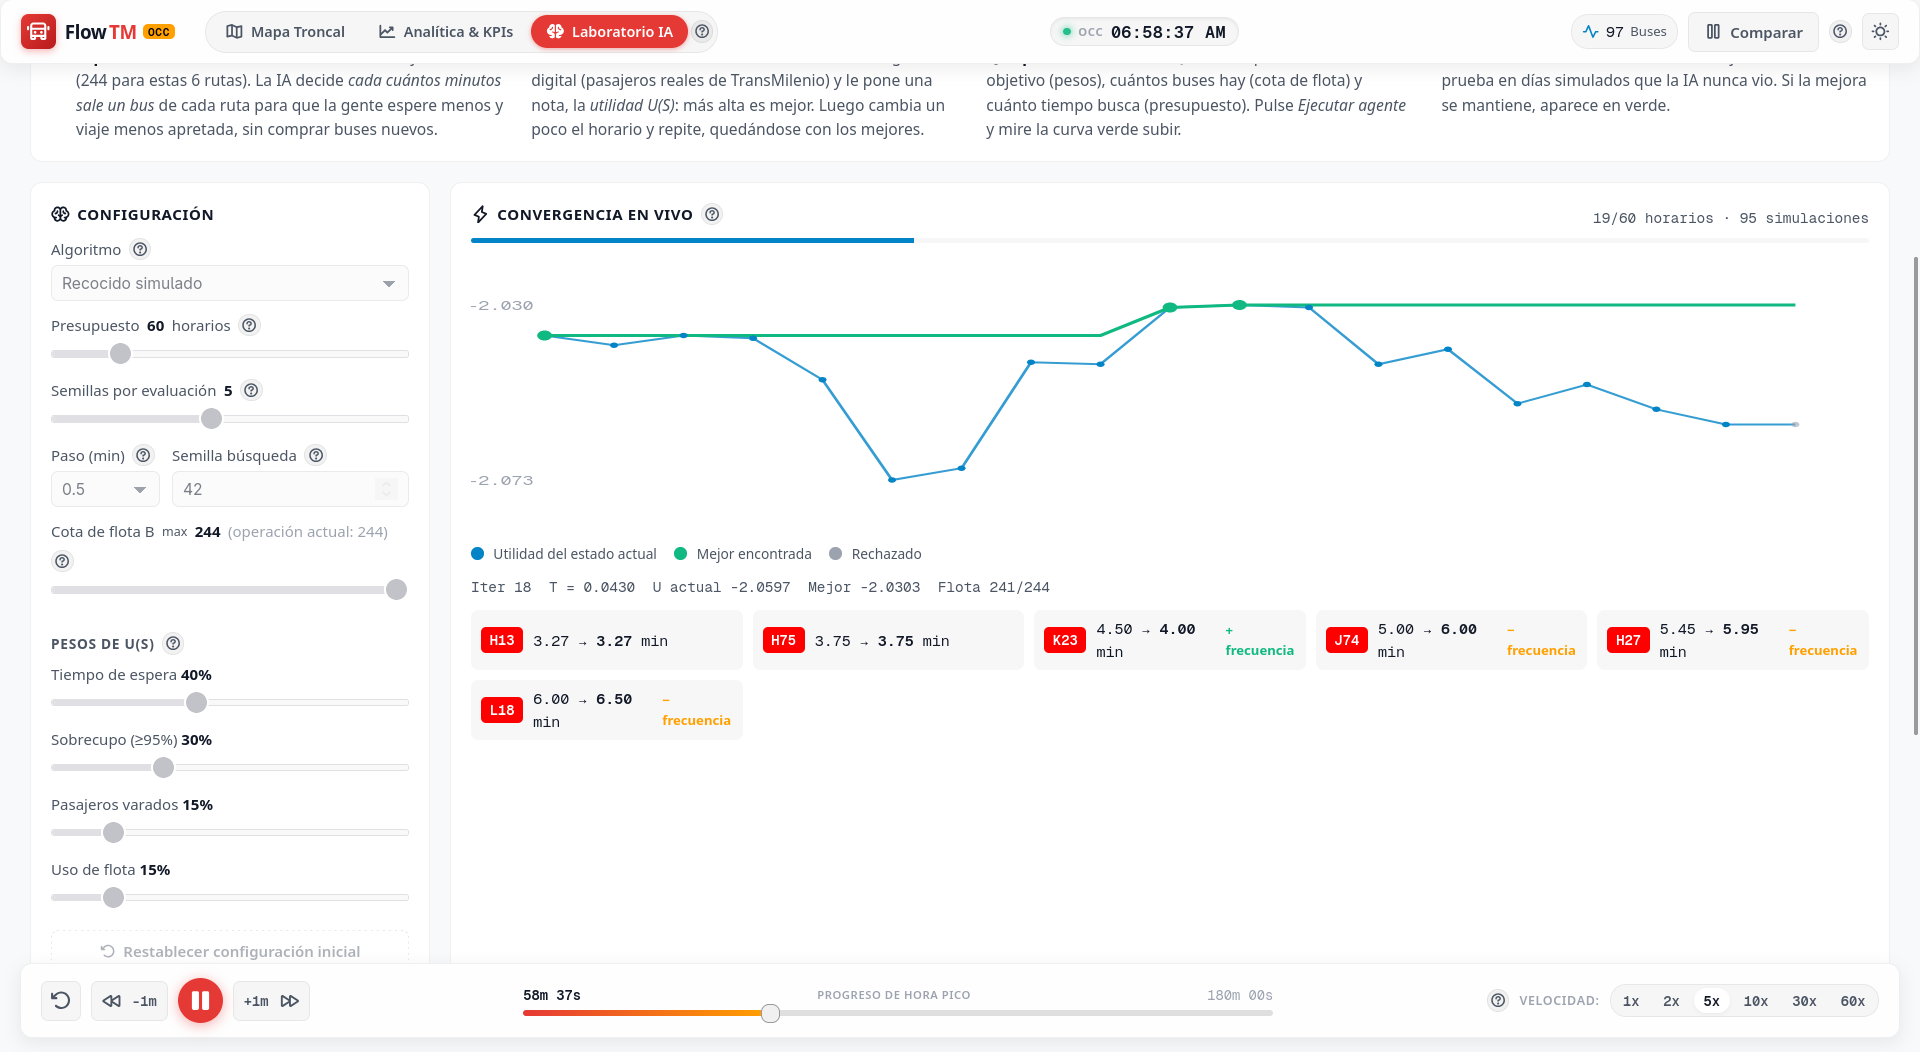
\includegraphics[width=\textwidth]{img/dash-2.png}
        \caption{Simulador de optimización}
        \label{simulador}
      \end{figure}
      


      \begin{block}{CONCLUSIONES}

        \begin{itemize}
          \item La redistribución de frecuencias reduce el sobrecupo en el escenario simulado y mejora la utilidad multicriterio.
          \item La validación fuera de muestra no demuestra una reducción de la espera media; el resultado es un compromiso entre ocupación, espera y flota.
          \item Las conclusiones dependen de la demanda reconstruida, la capacidad asumida y el corredor estudiado; se requiere validar otros corredores y condiciones operativas.
          \item Se construyó un simulador y visor de rutas tanto de Transmilenio original como las propuestas por el agente, facilitando una comparativa entre ambas rutas.
        \end{itemize}

      \end{block}

      \begin{block}{REFERENCIAS BIBLIOGRÁFICAS}

        \begin{thebibliography}{99}

          \bibitem{gtfs}
          MobilityData. \textit{General Transit Feed Specification (GTFS) Reference}. 2026.
          \url{https://gtfs.org/documentation/schedule/reference/}

          \bibitem{transmilenio}
          TransMilenio S.A. \textit{Portal de Datos Abiertos: GTFS estático y validaciones del componente troncal}. 2026.
          \url{https://datosabiertos-transmilenio.hub.arcgis.com/}

          \bibitem{newell}
          Newell, G. F. \textit{Applications of Queueing Theory}. 2nd ed. Chapman and Hall, 1982.
          DOI: \url{10.1007/978-94-009-5970-5}.


        \end{thebibliography}


      \end{block}

      \begin{block}{Agradecimientos}

        TODO

      \end{block}

    \end{column}
    \separatorcolumn



  \end{columns}
\end{frame}

\end{document}
